\subsubsection*{Architecture}
An overall design and architecture was created in the early sprints of the project.
 The server side software is different from the rest of the software made in the multi project group, as the customers will never actually see it in action. It works as intended if they never notice it is there.
Almost all requirements from our customers concern the user interface and general feel of the GIRAF apps. In regards to the server software, it is the requirements of the multi project that are of interest,
in particular Oasis, as their responsibility is to link the GIRAF apps to Savannah.

The GIRAF system is designed in such a way that it deploys with two databases: Savannah - our project, a global database for a full deployment unit, and Oasis - or localDB, a local database which exists only
on the mobile devices, which has an almost identical schema to Savannah's database.
Rather than having Oasis query the global database directly, it was decided to implement access to both the databases through a software layer, as shown in \autoref{fig:softwareLayers}.
The pros and cons of this seemingly redundant software layer was considered, see \autoref{table:proconSoftwareLayers}

\begin{figure}[H]
	\centering
		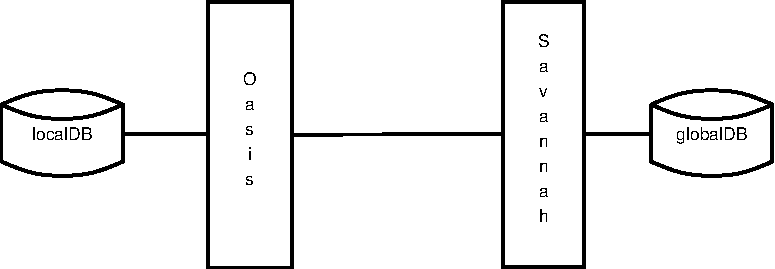
\includegraphics[scale=1]{images/softwareLayers}
	\caption{Software layers}
	\label{fig:softwareLayers}
\end{figure}

\begin{table}[H]
  \begin{center}
    \begin{tabular}{c|c}
    Pros                   &             Cons \\
    \hline
    More flexibilty        & Higher complexity\\
    Independent DB updates & Lower performance\\
    \end{tabular}
    \caption{Pros and cons of an extra software layer between the databases}
    \label{table:proconSoftwareLayers}
  \end{center}
\end{table}

Having an extra software layer between the databases means we can alter the global and local databases independently of each other. By providing software with methods for extracting specific
details from Savannah, like full profiles, Oasis does not have worry about Savannah's internal database schema. The downside of this is that the complexity inevitably will be higher, and performance
will be lower. The performance issue is not critical though, since the perceived performance of the system will be dominated by the bandwidth of the mobile devices. 
The communication between the software layers will be facilited by the sw6ml XML language, presented in \autoref{sw6ml}

Savannah has a three layered internal architecture, show in \autoref{figure:savaArch}.

\begin{figure}[H]
  \centering
    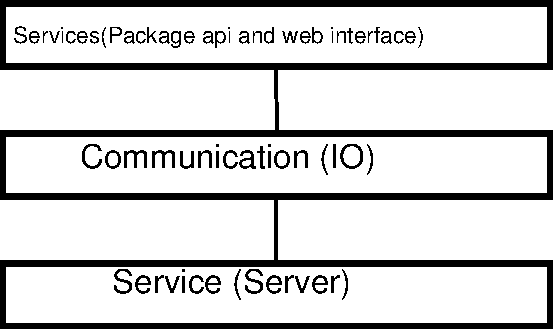
\includegraphics{images/savaArch}
  \caption{Savannah's architecture}
  \label{figure:savaArch}
\end{figure}

A short description of each layer's responsibilities follows:

\begin{description}
 \item[Services] The services layers consists of the services that we provide to external users. We have considered two services to include, which are an API for creating transmissions packages	 		that Savannah understands, and the web interface discussed in \autoref{sect:webInterface}.
 \item[Communication] The communication layer consists of the IO package of the server side software, which handles retrieval and responding.
 \item[Service] The service layer consists of event handling, query handling and the building of sw6ml documents.
\end{description}


\subsubsection*{Design}
The overall server software is designed around a producer-consumer pattern, where Oasis acts as the producer through Savannah's IO layer.
Request or commit packages sent to Savannah will be processed by the \code{IOHandler}, which will add an event to the \code{EventQueue}. The consumer is the server itself, which will remove events from the queue and process its content, being it a request or a commit. Using a queue based design was chosen for the sake of simplicity. The project is a part of learning process, and building a server with concurrent event handling was down prioritized versus a simpler server, which would allow us to gain experience and still meet the requirements of the study regulations.
 A draft of the design for the server can be seen in \autoref{figure:serverMockup}. This diagram represents the general idea and flow of the server, and should not be understood as formal technical specification.
\begin{figure}[H]
 \centering
  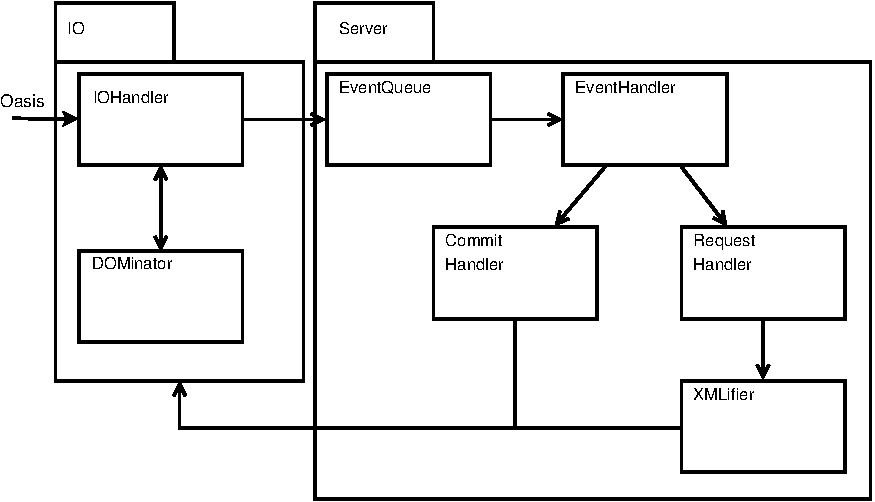
\includegraphics[scale=1]{images/savaIniDesign}
 \caption{Savannah server draft}
 \label{figure:serverMockup}
\end{figure}
